\begin{frame}
\frametitle{Introduction: Bose-Bose miscible mixture without buoyancy}
\setbeamercovered{invisible}


\begin{columns}[t]
\column{0.8\linewidth}
\begin{itemize}
\item 2-component BEC: 2 Zeeman levels $\ket{\uparrow}$, $\ket{\downarrow}$
\item Caracterized by scattering lengths:
	\begin{itemize}
		\item Intracomponent: $a_{\uparrow\uparrow}$, $a_{\downarrow\downarrow}$
		\item Intercomponent: $a_{\uparrow\downarrow}$
	\end{itemize}
\item Important property: miscibility if $a_{\uparrow\downarrow}<\sqrt{a_{\uparrow\uparrow}a_{\downarrow\downarrow}}$
\end{itemize}	
\column{0.2\linewidth}


\begin{figure}
\centering
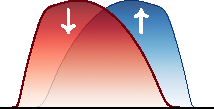
\includegraphics[scale=0.7]{Figures/Spinor_Illustration.pdf}
\end{figure}

\end{columns}

\begin{itemize}
\item Even when miscible: buoyancy problem in harmonic trap when $a_{\uparrow\uparrow} \neq a_{\downarrow\downarrow}$
\item It prevents the study of the static and dynamic response in harmonic trap
\end{itemize}
\begin{itemize}
\item Our system: $|3^2S_{1/2}, F=1, m_F=\pm1\rangle$ states of sodium 
\begin{figure}
\centering
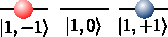
\includegraphics[scale=1.2]{Figures/Spinor_Scheme.pdf}
\end{figure}
\item Advantages
	\begin{itemize}
		\item Miscible
		\item Without buoyancy $a_{\uparrow\uparrow} = a_{\downarrow\downarrow} \equiv a$ 
		\item Close to the miscible/immiscible phase transition $(a-a_{\uparrow\downarrow})/a=0.07 \ll 1$
	\end{itemize}
\item Goals
\begin{itemize}
		\item Study the linear and dynamic response
		\item Observe that these properties are drastically modified close to the phase transition despite the weakly interacting nature of the gas
	\end{itemize}
\end{itemize}


\end{frame}
